\begin{chapter}{The TVMT Library}
\label{ch:library}

The library which was developed in the course of this work is an easy-to-use, fast C++14 template library for TV minimization of manifold valued two- or three-dimensional images.

\section{Capabilities} % (fold)
\label{sec:Capabilities}
\subsection{Supported Manifolds} % (fold)
\label{sub:Supported Manifolds}
\begin{itemize}
    \item Real Euclidian space $\mathbb{R}^n$
    \item Sphere $S^n=\left\lbrace x\in\mathbb{R}^{n+1}:\; \norm{x}=1\right\rbrace$
    \item Special orthogonal group $SO(n)=\left\lbrace R\in\mathbb{R}^{n\times n}:\; RR^T=\mathbbm{1}, \operatorname{det}(R)=1 \right\rbrace$
    \item Symmetric positive definite matrices $SPD(n)=\left\lbrace S\in\mathbb{R}^{n\times n}:\; S=S^T, x^TSx>0\; \forall x\in\mathbb{R}^n \right\rbrace$
    \item Grasmann manifold $Gr(n,p)=$
\end{itemize}
% subsection Supported Manifolds (end)

\subsection{Data} % (fold)
\label{sub:Data}
\begin{itemize}
	\item 2D and 3D images
	\item Input/Output via OpenCV integration supporting all common 2D image formats
	\item CSV input for matrix valued data
	\item Input methods for raw volume image data as well as the NIfTI \cite{nifti} format for DT-MRI images
	\item Various methods to identify damaged areas for inpainting
\end{itemize}
% subsection Data (end)

\subsection{Functionals} % (fold)
\label{sub:Functionals}
\begin{itemize}
    \item isotropic(only possible for IRLS) or anisotropic TV functionals
    \item first order TV term
    \item weighting and inpainting possible
\end{itemize}
% subsection Functionals (end)

\subsection{Minimizer} % (fold)
\label{sub:Minimizer}
\begin{itemize}
	\item IRLS
	\item PRPT
\end{itemize}
% subsection Minimizer (end)

\subsection{Visualizations} % (fold)
\label{sub:Visualizations}
\begin{itemize}
    \item OpenGL rotated cubes visualization for SO(3) images
    \item OpenGL ellipsoid visualization for SPD(3) images
    \item OpenGL volume renderer for 3D volume images
\end{itemize}
% subsection Visualization (end)

% section Capabilities (end)

\section{Design concepts} % (fold)
\label{sec:Design}

\subsection{Goals} % (fold)
\label{sub:Goals}

\subsubsection{Performance} % (fold)
\label{ssub:Performance}
Since the core parts of the implementation are originally based on a matlab prototype by Sprecher \cite{SprecherIRLS}, \cite{manuel} and \cite{mara}, one of the most important
goals was of course a faster implementation with a smaller memory footprint. On the test platform with two hyperthreaded 2.8GHz cores Intel i5-2520 with AVX vector extensions
the Matlab implementation froze for images larger than one Megapixel(MP). Hence, the C++ implementation should enable the algorithm to be tested in a much broader scope which is
also closer to common picture sizes in image processing, especially since even smartphones today easily produce pictures in the Megapixel range.
In additions to that, also other factors affecting the performance of the algorithm, such as cache locality and memory speed, can be investigated.\\

The main performance driver for this library is the multilevel-parallelization. Evidently, this does not include the formulation of the IRLS minimization algorithm itself, due to the fact that
it is naturally a iterative method, but rather any possible subtask such as computation of the functional values, gradient and Hessian, for example. On top of that, we tried to
maximize cache locality on the loop level and to free memory as soon as possible but keep data that is used very often and requires costly recomputation, like for example the IRLS weights.\\ 

In contrast to the original Matlab implementation, the computation of various quantities such as weights, first and second derivatives is not realized with tensor products any more.
For Matlab, due the low speed of its internal loop constructs, the approach is justified but in a pure C++ implementation other factors are more important.
One reason for the change is improved readability and maintainability of the code since tensor product usualluay tend to become very convoluted,
especially for the manifolds with matrix representations. Also the modularization of the manifold class is not straightforward any more.\\
From a performance and parallelization perspective, contractions of tensor products are similar to Matrix products and usually require some sort of blocking scheme for parallelization.
In addition to that, because certain reshapes of the image container prior to the computation are necessary, the dimensions to be summed over are not necessarily contiguous in memory
such that a high a cache utilization is more difficult to achieve.\\
Finally, in order to formulate certain operations as tensor products, temporary tensors of the correct dimensionality need to be created, which are actually not necessary.\\

Another measure that significantly reduces the memory footprint for the IRLS minimizer, especially for manifolds with matrix representations, is to only save gradient and hessian
in their local tangent space basis representation, such that the degrees of freedom correspond the intrinsic manifold dimension not the dimension of the embedding space. This also reduces
the time to solve the sparse linear system.\\
% subsubsection Performance (end)

\subsubsection{Modularization and Extendability} % (fold)
\label{ssub:Modularization}
In principle the programming paradigm in Matlab is still procedural resulting in a hierarchy of functions for the various tasks. Handling different types of manifolds
then usually requires \texttt{switch} expressions in all functions that use manifold-specific functionality. Adding a support for a new manifold to the algorithm or modifying
existing manifold functionalty makes a modification of all \texttt{switch} cases necessary. There is no single point of change but many source files need to edited.\\

For the TVMT Library an object oriented and generic programming approach was chosen, which tries to model each variable component of the algorithm in a separate class, as 
independent of the other components as possible. Differences in each class are represented by specializations of their primary class template. The best example for that is the
manifold class which has a specialization for every supported manifold type and due to the fact that the functions implemented in those class specializations are generally
just functions of one or two elements of the manifold, they could also be used in other projects which require the same functionality.\\

Interfaces between classes are provided by giving classes higher in the hierarchy template parameters corresponding to lower classes: The class modelling the functional, for instance,
has a manifold type template parameter, as described in more detail in the section \ref{sec:Components}. Like all other component classes, also the functional class can be extended
by adding further specializations for other types of functionals, that include for example higher order terms or have different fidelity terms \cite{opticalflow}.\\

Those specializations also have the advantage that the code is just in one file, a single point of change to increase readability and maintainability.
% subsubsection Modularization (end)

% subsection Goals (end)

\subsection{Levels of parallelization} % (fold)
\label{sub:Levels of parallelization}
Parallelization takes place on two levels. The first one is shared memory multithreading implemented with the OpenMP language extensions. In most cases this is realized 
using the so-called \textit{pixel-wise kernels} of the VPP library, which makes it possible to map an arbitrary function on all pixels of a set of image containers: The function is
called for each tuple of pixels having the same coordinates in their respective image. For the parallel execution each processor is assigned a batch of image rows.
If the pixel wise kernels are not applicable, for example if the needed subdomain of the image is too complicated, we use manual OpenMP loop parallelization. At the
time of writing, this unfortunately also includes 3D images, such that we implemented an own version of 3D pixel-wise kernels to keep the code compact.\\

The alternative to the above described tensor product implementation is to use pixel-wise kernels to parallelize any operation to requires iteration over an image container.
For most computations, in the case of computing derivatives, we only need the pixel and its next neighbor in a given dimension. For calculating the forward derivatives we just 
to have call the pixel-wise kernel with two subimages of our current working image: One with the last slice (of the given dimension) missing and one with the first slice missing.
This is demonstrated by the following short listing \ref{code:pixelwise_demo} and further illustrated in \ref{fig:pixelwise_kernel}:\\

\cppinline
\begin{lstlisting}[label=code:pixelwise_demo,caption={Pixel-wise forward derivative computation}]
auto calc_first_arg_deriv = [&] (value_type& x, const weights_type& w, const value_type& i, const value_type& n) { MANIFOLD::deriv1x_dist_squared(i, n, x); x *= w; }; 

img_type YD1 = img_type(without_last_row);
vpp::pixel_wise(YD1, weightsY_ | without_last_row, data_.img_ | without_last_row, data_.img_ | without_first_row) | calc_first_arg_deriv;
\end{lstlisting}

\begin{figure}[h!]
        \centering
	    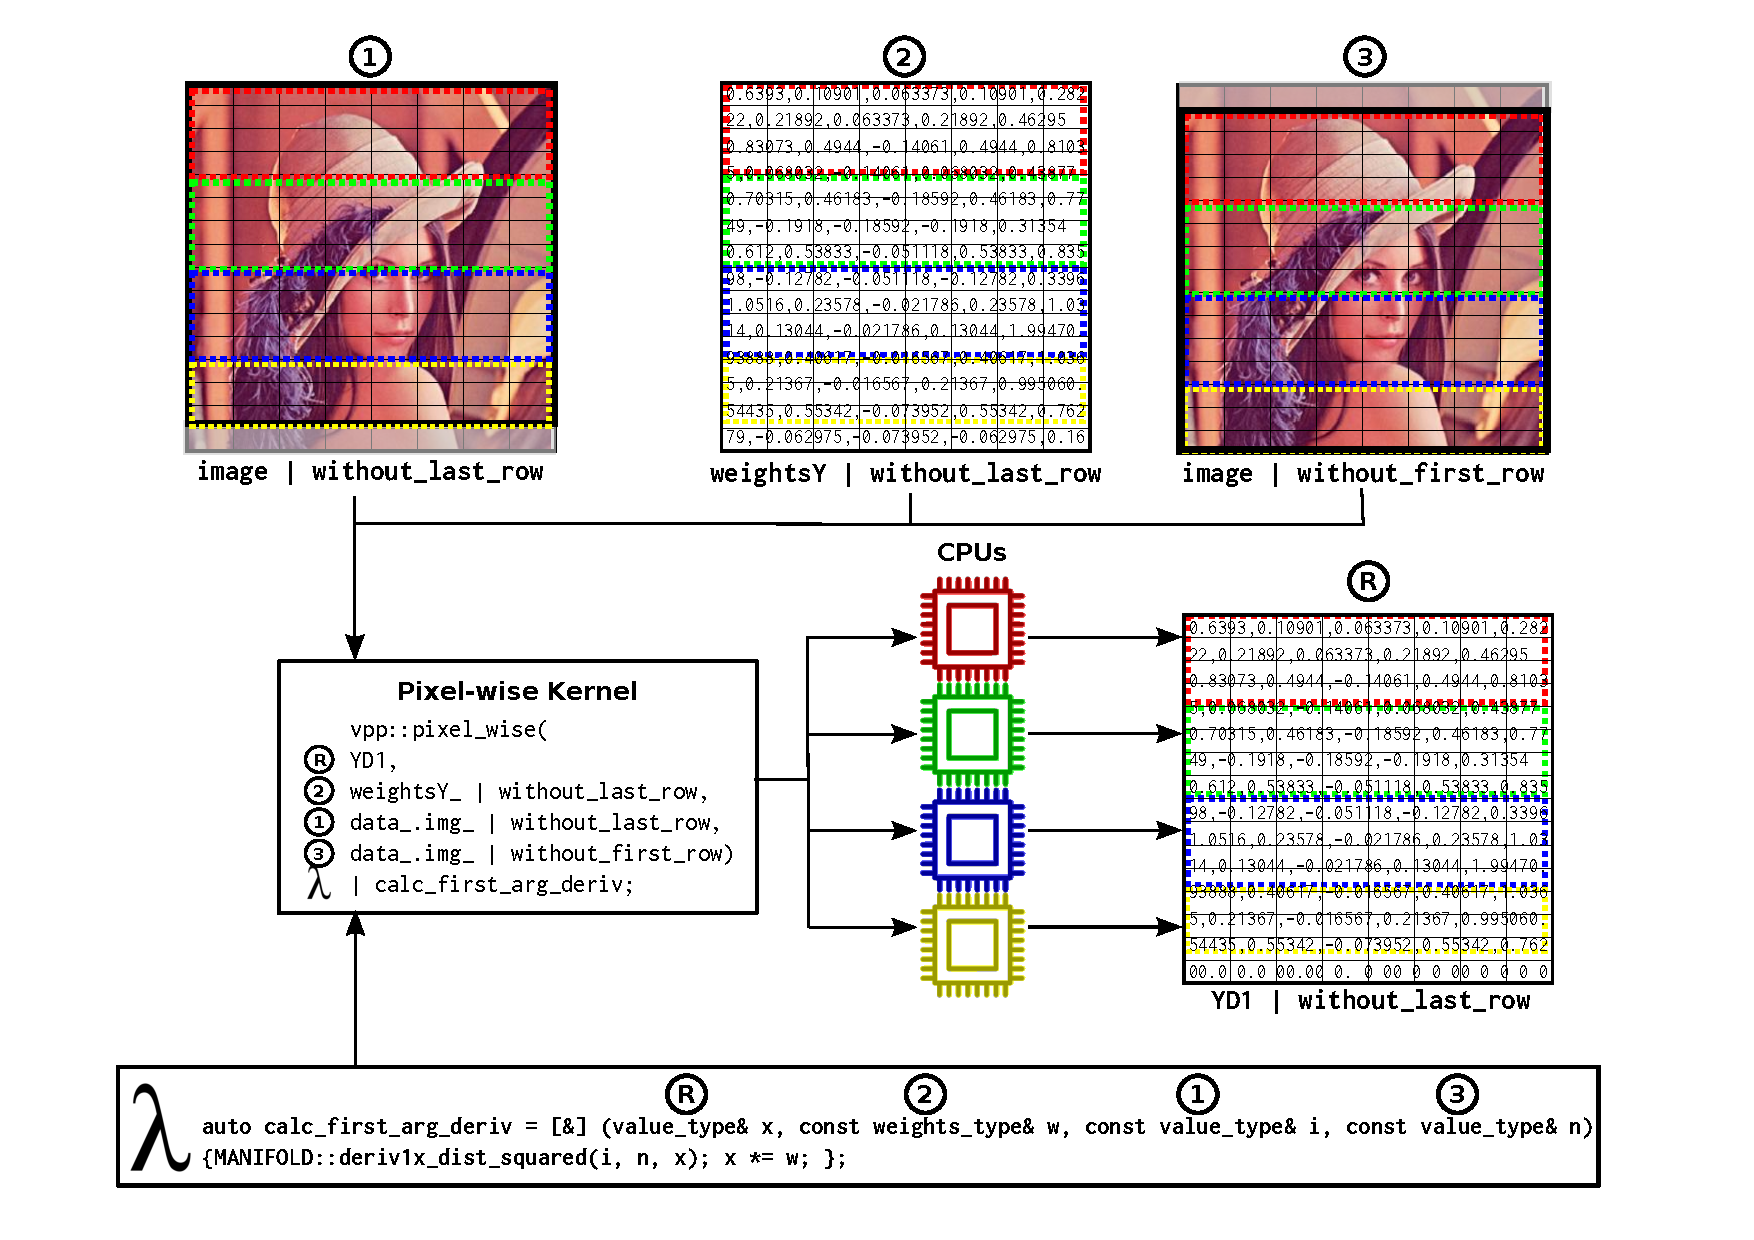
\includegraphics[width=1.0\linewidth]{./figures/library/pixelwise_kernel.pdf}
	\caption[Calculation using pixel-wise kernels]{Parallel calculation of derivatives in $y$-direction and weighting using pixel-wise kernels.
	    For each pixel position $(i,j)$ in the three input pictures, \circnum{1}, \circnum{2} and \circnum{3}, as well as the output picture
	    \circnum{R} the pixel-wise kernel creates a tuple $(R_{ij}, 2_{ij}, 1_{ij}, 3_{ij})=(\text{YD1}_{i,j},\text{weightY}_{i,j},\text{Image}_{i,j},\text{Image}_{i,j+1})$
	    which is than used to call the specified lambda function. Depending on the row number of the pixel, the calls are executed by different CPU cores.
	}
	\label{fig:pixelwise_kernel}
\end{figure}

The advantage is that even though we evaluate some function for a pair of neighboring pixels which are not adjacent in memory, the parallel processing is still
always row-wise. Since rows in row major languages like C++ are contiguous in memory we can avoid frequent memory access on distant locations and consequently avoid cache thrashing to a
certain degree.\\

The second level of parallelization is instruction level parallelism, also known as \textit{Single Instruction Multiple Data} (SIMD), which uses the
processor's vector extensions (e.g. SSE, AVX, NEON).
The CPU provides some additional special SIMD registers with increased size of usually 128 bits to 512 bits such that multiple integer or floating point variables fit inside.
Then an arithmetic operation is simultaneously applied to all variables in the register (see figure \ref{fig:simd}) such that theoretically the amount of floating point operations is multiplied by the number
of variables fitting in the registers. \\

\begin{figure}[h!]
        \centering
	    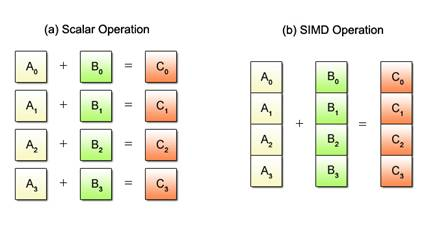
\includegraphics[width=0.7\linewidth]{./figures/library/simd.jpg}
	\caption[SIMD parallelization]{Instruction level parellelism using SIMD registers.
	}
	\label{fig:simd}
\end{figure}

In order to really achieve this speedup the data must be aligned in memory which means the address of pixels in memory must always be multiple of the SIMD register size. Fortunately,
that issue is handled by the VPP and Eigen libraries enabling the compiler to perform the necessary vectorization optimizations.

% subsection Levels of parallelization (end)


\subsection{C++ techniques} % (fold)
\label{sub:C++ techniques}
The TVMT Library tries to take advantage of new C++11 and C++14 language features in order to speed up computations via compile-time optimizations and also make the code
more compact and readable. The most important tools in that regard are lambda functions and variadic templates which are shortly described in the following section.

\subsubsection{Lambda functions} % (fold)
\label{ssub:Lambda functions}
A lambda function is basically a locally defined function object, which is able to capture variable from the surrounding scope that can but need not to be named.
The corresponding Matlab language construct is an anonymous function or function handle, usually defined using the @ operator. The following listing
shows the basic definitions and uses cases of lambda functions:\\

\cppinline
\begin{lstlisting}[label=code:lambdafun,caption={Lambda functions}]
int init = 5;
std::vector<int> v {1, 2, 3, 4};

// C++11 lambda function for adding integers
// init is captured by reference
auto f = [&] (int a, int b) {return a + b + init;};

// C++14 generic argument lambda function
// init is captured by value
auto g = [=] (auto a, auto b) {return a + b + init;};

//Call named lambda functions
int d = f(8, 3);
double e = g(1.0f, 5);

// or directly pass anonymous lambda function as argument
std::transform(v.begin(), v.end(), v.begin(), [] (auto x) { ++x; });
\end{lstlisting}

In the TVMT library lambda functions provide the connection between the static manifold methods and the pixel-wise kernels which apply them to the image containers.
A typical case can be seen in the already introduce listing \ref{code:pixelwise_demo}. Since lambda functions are only locally defined, in the scope where they are actually needed,
one can avoid making the method list of the classes unnecessary long.
% subsubsection Lambda functions (end)

\subsubsection{Variadic templates} % (fold)
\label{ssub:Variadic templates}
With variadic templates it is possible to define functions which take a variable number of arguments. Obviously, this is also possible in other languages like Matlab or
C with the most prominent example being the function \texttt{printf}. However this usually implemented using some list type (in C \texttt{va\_list} ), which adds additional 
overhead, whereas in C++ it is realized via some special kind of template metaprogramming which is recursive in nature. The recursion, in turn, is resolved at compile-time
an leads to code that is actually equivalent to manually defining a function with the desired number of arguments and consequently there is no additional runtime effort.\\

\cppinline
\begin{lstlisting}[label=code:variadic,caption={Variadic template example}]
// Recursion base case
template<typename T>
T sum(T v) {
    return v;
}

// Recursive template
template<typename T, typename... Args>
T sum(T first, Args... args) {
    return first + sum(args...);
}
\end{lstlisting}

The main application for this constructs in TVMTL are the implementation of the Karcher mean, needed for the proximal point implementation, and TVMTL's own version
of the 3D pixel-wise kernels.

% subsubsection Variadic templates (end)
% subsection C++ techniques (end)
% section Design (end)

\section{Components} % (fold)
\label{sec:Components}

\subsection{Manifold classes} % (fold)
\label{sub:Manifold classes}
The manifold template class encapsulates all information and methods related to the differential geometric structure of the data. 
This enables the generic implementation of the functionality higher in the class hierarchy such as functional evaluations or minimizers.
The primary template has the following parameters
\cppinline
\begin{lstlisting}
// Primary Template
template <enum MANIFOLD_TYPE MF, int N, int P=0>
struct Manifold {
}; 
\end{lstlisting}
where \texttt{MF} is an enumeration constant to specify the type of the manifold, $N$ denotes the dimension of the representation space and $P$ the dimension of subspaces,
as in the case of Grassmann manifolds. In order to add a new manifold one just has to implement a specialization of this primary template.\\

So far, the manifold classes contains functionality necessary for TV minimization using either the IRLS or proximal point algorithm and furthermore some additional operations
that are needed for supporting tasks like interpolation and smoothing. The classes are implemented using only static constants and methods: At no time is it necessary or 
desired to actually instantiate the class. The methods itself are usually unary or binary functions, with parameters and result all passed by reference to avoid copies.
Since these methods are called very often, basically for every pair of neighboring pixels, they are all declared \texttt{inline} in order to support the compiler during 
the code optimization.\\

It is also possible to use these classes in other projects requiring similiar functionality like 
for instance when implementing a geodesic finite element solver.\\

In the following we will look at excerpts of the SPD implementation to illustrate which information and functionality a new manifolds class need to provide and to give an overview
of the available functions.

\subsubsection{Static constants} % (fold)
\label{ssub:Static constants}
\cppinline
\begin{lstlisting}
static const MANIFOLD_TYPE MyType;	// SPD
static const int manifold_dim ;		// N*(N+1)/2
static const int value_dim;		// N*N

static const bool non_isometric_embedding;
\end{lstlisting}
The first constant just stores the manifold template template parameter introduced above, while \texttt{manifold\_dim} and \texttt{value\_dim} are the intrinsic dimension of the manifold
and of its embedding space, respectively. Finally, the boolean constant is just a flag which tells the algorithm that special pre- and postprocessing for interpolation is necessary.\\
% subsubsection Static constants (end)

\subsubsection{Type definitions} % (fold)
\label{ssub:Type definitions}
To enable the generic formulation of the algorithms the manifold classes provide a mapping between the types of their values, derivatives, tangent bases and underlying scalar type and their 
actual representation as matrix and vector data types of the Eigen linear algebra library. Examples can be seen in the following listing:

\cppinline
\begin{lstlisting}
// Scalar and value typedefs
typedef double scalar_type;
typedef double dist_type;
typedef Eigen::Matrix<scalar_type, N, N> value_type;
// ...

// Tangent space typedefs
typedef Eigen::Matrix <scalar_type, N*N, N*(N+1)/2> tm_base_type;
// ...

// Derivative Typedefs
typedef value_type deriv1_type;
typedef Eigen::sMatrix<scalar_type, N*N, N*N> deriv2_type;
typedef Eigen::Matrix<scalar_type, N*(N+1)/2, N*(N+1)/2> restricted_deriv2_type;
// ...
\end{lstlisting}
% subsubsection Type definitions (end)

\subsubsection{Static methods} % (fold)
\label{ssub:Static methods}
Finally, the following methods are implemented for the manifold classes

\begin{description}
    
    \item[Riemannian distance function and its derivatives] \hfill \\
	\cppinline
	\begin{lstlisting}
inline static dist_type dist_squared(cref_type x, cref_type y);
// First derivatives	    
inline static void deriv1x_dist_squared(cref_type x, cref_type y, deriv1_ref_type result);
inline static void deriv1y_dist_squared(cref_type x, cref_type y, deriv1_ref_type result);
// Second derivatives
inline static void deriv2xx_dist_squared(cref_type x, cref_type y, deriv2_ref_type result);
inline static void deriv2xy_dist_squared(cref_type x, cref_type y, deriv2_ref_type result);
inline static void deriv2yy_dist_squared(cref_type x, cref_type y, deriv2_ref_type result);
	\end{lstlisting}
    
    \item[Exponential and Logarithm map] \hfill \\
	\cppinline
	\begin{lstlisting}
template <typename DerivedX, typename DerivedY>
inline static void exp(const Eigen::MatrixBase<DerivedX>& x, const Eigen::MatrixBase<DerivedY>& y, Eigen::MatrixBase<DerivedX>& result);
inline static void log(cref_type x, cref_type y, ref_type result);

inline static void convex_combination(cref_type x, cref_type y, double t, ref_type result);
	\end{lstlisting}

	The parameters of the exponential here are not the manifolds own typedefs but the base class of all Eigen matrix data types. The reason for using this construction is that the function
	can also be called with composite expressions (e.g. $XY+Z$) without a temporary copy. Most of the other functions are usually called with atomic expression only, hence there is no
	need to use this more complicated construction on a general basis.\\
	The \texttt{convex\_combinations} method denotes a point $z$ on the manifold by following a unit time geodesic connecting the points $x$ and $y$ for a time $t$.

    \item[Karcher means] \hfill \\
	\cppinline
	\begin{lstlisting}
inline static void karcher_mean(ref_type x, const value_list& v, double tol=1e-10, int maxit=15);
inline static void weighted_karcher_mean(ref_type x, const weight_list& w, const value_list& v, double tol=1e-10, int maxit=15);

// Variadic templated version
template <typename V, class... Args>
inline static void karcher_mean(V& x, const Args&... args);
	\end{lstlisting}
	
	Implementations for finding the Karcher mean of an arbitrary number of points. The first version requires the points to be stored in a \texttt{std::vector} container while
	the second version is based on variadic templates and expects the arguments just as a comma separated list after the first argument, where the final result will be stored.
	Creating the list for the first version eventually requires copying and is consequently slower but has an overloaded version which allows to compute a weighted Karcher mean
    
    \item[Tangent plane basis, projector and interpolation] \hfill \\
	\cppinline
	\begin{lstlisting}
// Basis transformation for restriction to tangent space
inline static void tangent_plane_base(cref_type x, tm_base_ref_type result);
// Projection
inline static void projector(ref_type x);
// Interpolation pre- and postprocessing
inline static void interpolation_preprocessing(ref_type x);
inline static void interpolation_postprocessing(ref_type x);
	\end{lstlisting}

	The first function computes a basis of the tangent space at the point $x$ and stores it in \texttt{result} as the columns of a matrix.\\
	The projector, if defined for the given manifold, will project a point of the ambient embedding spacing onto the manifold. In the case of Euclidian space, where the 
	embedding space and the manifold are identical, this function does nothing and will be optimized out by the compiler. Nevertheless, it must exist or programs will not compile.\\
	Interpolation pre- and postprocessing is necessary for instance for the SPD manifold. Other manifolds must just provide an empty implementation.
\end{description}
% subsubsection Static end)
% subsection Manifold classes(end
\subsection{Data class} % (fold)
\label{sub:Data class}
The data class handles anything related to storage, input and output of two- or threedimensional image data, as well as some support functions for detecting edges and damaged areas in a picture.
In contrast to the manifold class, the data class needs to be instantiated such that a reference to the data object can be passed to any class which needs data access. In turn, in addition
to the dimension of the picture, the data class takes a fully specialized manifold class type as a template parameter:

\cppinline
\begin{lstlisting}
// Primary Template
template <typename MANIFOLD, int DIM >
class Data {
};    
\end{lstlisting}

There are basically four multi-dimensional arrays stored in the data class: The original noisy image, the current working image and, if applicable, arrays storing the inpainting
and edge weight information. For storage, the n-dimensional VPP \cite{VPP} image container is used.\\

This image container class works very well together with the Eigen vector and matrix data types, provides a variety of expressive loop- and iterator constructs and also takes care
of the alignment of the image data in memory, which is a prerequisite for the \textit{Single Instruction Multiple Data} (SIMD) optimization and vectorization by the compiler.
Since the memory management of the container is based on \texttt{std::shared\_pointer} it is also very easy to efficiently access subimages or slices of an image without any copies.\\

The most common input method for 2D and 3D are summarized in the following code snippet:
\cppinline
\begin{lstlisting}
 // 2D Input functions
void rgb_imread(const char* filename);	// for R^3
void rgb_readBrightness(const char* filename); // for R
void rgb_readChromaticity(const char* filename); // for S^2
void readMatrixDataFromCSV(const char* filename, const int nx, const int ny);

// Synthetic SO/SPD picture 
void create_nonsmooth_son(const int ny, const int nx);
void create_nonsmooth_spd(const int ny, const int nx);
 
//3D Input functions
void rgb_slice_reader(const char* filename, int num_slides); 
void readMatrixDataFromCSV(const char* filename, const int nz, const int ny, const int nx);
void readRawVolumeData(const char* filename, const int nz, const int ny, const int nx);
\end{lstlisting}
The purpose and usage of most of these methods is self-explanatory. The CSV readers expect the data to be a linear list of pixels, where the components of each pixel are
comma-separated and row-wise flattened, such that each line of the input file contains exactly one pixel. The order of the list is also row-wise for 2D or slice- than row-wise for 3D images,
respectively. \\ 
The slice reader reads a series of images, following the filename scheme \texttt{filenameX.ext}, where \texttt{X} is the number of the slice to be read into an image cube at $z$-coordinate
\texttt{X}.
% subsection Data class (end)

\subsection{Functional class} % (fold)
\label{sub:Functional class}
In addition to fully specialized Manifold and Data class types (third and fourth template parameters),
there are three further template parameters that must be specified by the library user. The first one
is the order of the functional which refers to order of the highest differential operator in the TV term of the functional.
So far, only first order functionals are implemented which would correspond to setting \texttt{ord=FIRSTORDER} in the primary template shown below

\cppinline
\begin{lstlisting}
//Primary Template
template <enum FUNCTIONAL_ORDER ord, enum FUNCTIONAL_DISC disc, class MANIFOLD, class DATA, int DIM=2>
class Functional{
};
\end{lstlisting}

The second template parameters \texttt{disc} determines whether the isotropic or the anisotropic version is to be used. Please not that for the proximal point algorithm only
anisotropic is available. Finally, the last parameter specifies the dimensionality of the data. \\
The main purpose of the functional class is to provide methods for the computation of all functional-related quantities, such as evaluation of the functional, its gradient,
hessian and construction of a local basis of the tangent spaces. That also means that in the IRLS case the functional class stores sparse linear system that needs to solved
in each Newton step.\\

For users of the library, the most important methods are those for setting the $\lambda$ and $\epsilon^2$ parameters.
\cppinline
\begin{lstlisting}
inline param_type getlambda() const { return lambda_; }
inline void setlambda(param_type lam) { lambda_=lam; }
inline param_type geteps2() const { return eps2_; }
inline void seteps2(param_type eps) { eps2_=eps; }
\end{lstlisting}

Should it be necessary, it is also possible to access some of the enumerated quantities directly using
\cppinline
\begin{lstlisting}
// Evaluation functions
result_type evaluateJ();
void  evaluateDJ();
void  evaluateHJ();
 
void updateTMBase();

inline const gradient_type& getDJ() const { return DJ_; }
inline const sparse_hessian_type& getHJ() const { return HJ_; }
inline const tm_base_mat_type& getT() const { return T_; }
\end{lstlisting}
The functions in lines 2, 3 and 5 merely trigger a recomputation while the last three functions return references to these quantities.


% subsection Functional class (end)

\subsection{TV Minimizer class} % (fold)
\label{sub:TVMinimizer class}
For the TV Minimizer class it makes sense to consider the IRLS and proximal point implementation separately. The primary template is shown in the following code snippet.
\cppinline
\begin{lstlisting}
//Primary Template 
template <enum ALGORITHM AL, class FUNCTIONAL, class MANIFOLD, class DATA, enum PARALLEL PAR=OMP, int DIM=2>
class TV_Minimizer{ 
};
\end{lstlisting}
As in the previous cases we have to provide fully specialized manifold, data and also functional types. Again, the last parameter specifies the dimension of the data. Of the
remaining to \texttt{PAR} has the default value OMP which specifies the method of parellization, in this case the OpenMP language extensions. Other methods including just serial
execution could be added later. The remaining template parameter, \texttt{AL} specifies the minimizer to be used and can take the values \texttt{IRLS} or \texttt{PRPT} (Proximal point).\\

For IRLS, we have the following user interface\\
\cppinline
\begin{lstlisting}
void first_guess();		    // First guess for inpainting
void smoothening(int smooth_steps); // Simple averaging box filter
newton_error_type newton_step();    // perform one newton step
void minimize();		    // full minimization
\end{lstlisting}

while for proximal point we have\\
\cppinline
\begin{lstlisting}
use_approximate_mean(bool u) { use_approximate_mean_ = u; } // turn mean approximation on/off
void first_guess();					    // First gues for inpainting
 
void updateFidelity(double muk);			    // Update Fidelity part
void updateTV(double muk, int dim, const weights_mat& W);   // Update TV part

void geod_mean();	    // Calculate geodesic mean
void approx_mean();	    // approximate mean using convex combinations

void prpt_step(double muk); // perform one proximal point step
void minimize();	    // full minimization
\end{lstlisting}


% subsection TVMinimizer class (end)

\subsection{Visualization class} % (fold)
\label{sub:Visualization class}
This class provides visualizations of 3D volume data and so far SO(3) and SPD(3) visualizations by cubes and ellipsoids. If these are to be used in user code it is necessary to link
against OpenGL, GLUT and GLEW libraries, which is explained in more detail in section \ref{sub:CMakeCompilation}. The visualization classes have the following primary template.
\cppinline
\begin{lstlisting}
//Primary Template
template <enum MANIFOLD_TYPE MF, int N, class DATA, int dim=2>
class Visualization{
};
\end{lstlisting}

The class methods that are relevant to users of the libary are summarized here\\
\cppinline
\begin{lstlisting}
void saveImage(std::string filename);
void GLInit(const char* windowname);

void paint_inpainted_pixel(bool setFlag);
\end{lstlisting}

The important function here is \texttt{GLInit} which initializes the rendering of the data. If one intends to also save the image, on has to specify a filename using
\texttt{saveImage} \textit{before} calling \texttt{GLInit}. Finally, \texttt{paint\_inpainted\_pixel} just sets a flag which decides whether inpainted pixels are not painted
at all (\texttt{setFlag = false}, default value) or if they are visualized with the value they have at the time of rendering. Usually one wants to set this to \texttt{true}
after the minimization to show the results.\\
A full example to this is presented in section \ref{ssub:dti_tut}\\

\subsubsection{SO(3) Visualization} % (fold)
\label{ssub:SO(3) Visualization}
For the visualization of SO(3) data we just consider a unit volume cube centered at the origin of $\mathbb{R}^3$ with its front face normal vector parallel to the y-axis.
Then the rotation matrix representing the SO(3) element is applied to the cube. To break the $O_h \simeq S_4\times S_2$ symmetry of the cube, we give a different color to
every face.

\begin{figure}[h!]
        \centering
	    
\includegraphics[width=0.8\linewidth]{./figures/library/cubes.pdf}
	    \caption[SO(3) cube visualization]{SO(3) Visualization as oriented, colored cubes}
	\label{fig:cube_visualization}
\end{figure}
% subsubsection SO(3) Visualization (end)

\subsubsection{SPD(3) Visualization} % (fold)
\label{ssub:SPD(3) Visualization}
For three-dimensional SPD matrices we have six degrees of freedom, which in the case of DT-MRI pictures correspond to the diffusion coefficients in different directions.
Those can visualized by ellipsoids using three degrees of freedom for their orientation in space and the remaining three for length of its semi-axis.\\
Starting with the unit sphere centered at the origin again, we compute eigenvector and eigenvalues for every SPD matrix. Due to the SPD propery a full basis of eigenvectors
with positive eigenvalues always exists. The diagonal matrix formed by the vector of eigenvalues is applied as a scaling transformation of the coordinate axis. The matrix
whose columns are the computed eigenvectors can then be interpreted as a rotation (or principal axis transformation of the ellipsoid).\\
To avoid large size difference and overlaps between the ellipsoids we also normalize the eigenvalues using the mean diffusity $\mu$ defined by
\begin{equation}
    \mu = \frac{1}{3} \sum_{i=1}^{3}\lambda_i.
\end{equation}

Finally, the color is defined by normalizing the largest eigenvector, called the principal direction, and mapping its coordinates to the RGB colorspace, such that clusters of
similar orientations can be more easily visually distinguished.

\begin{figure}[h!]
        \centering
	    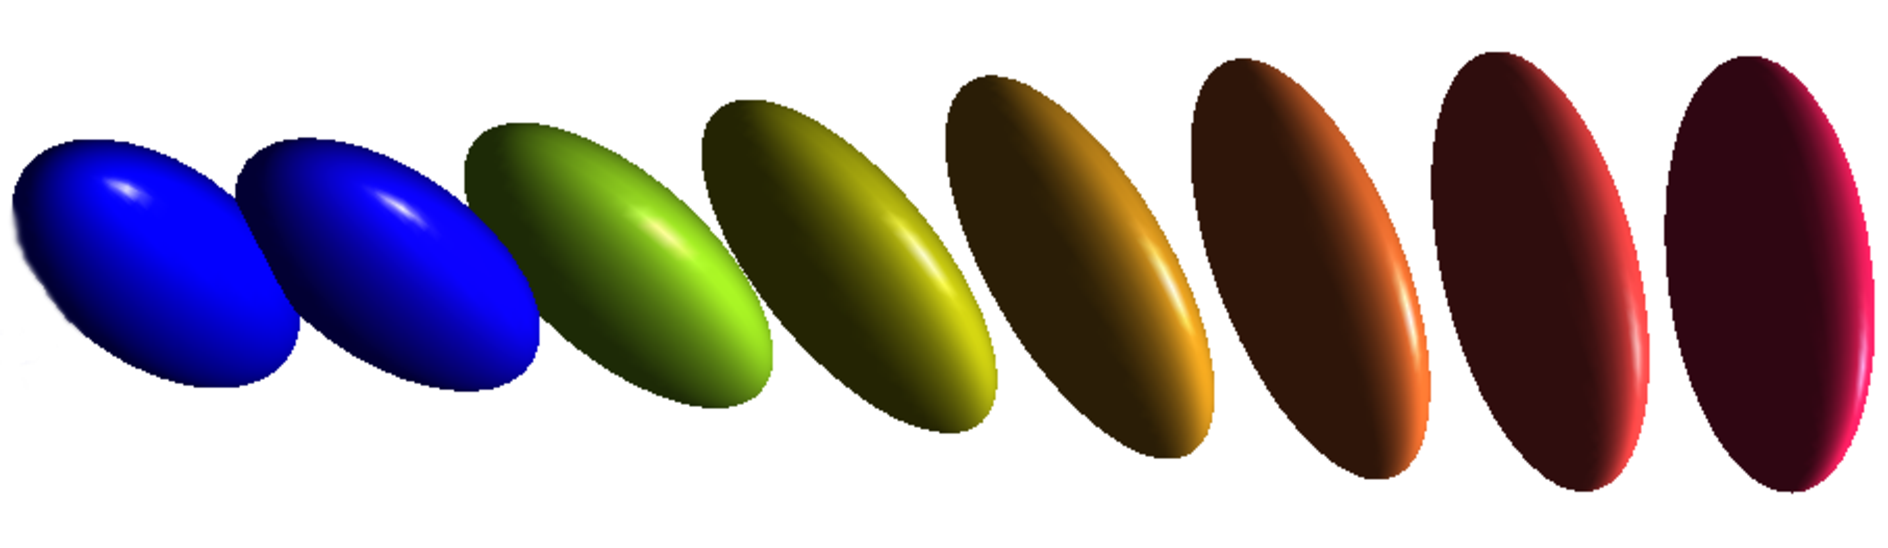
\includegraphics[width=0.8\linewidth]{./figures/library/ellipsoids.pdf}
	    \caption[SPD(3) ellipsoid visualization]{SPD(3) Visualization as oriented, colored ellipsoids}
	\label{fig:ellipsoid_visualization}
\end{figure}

In the case of 3D SPD images the rendering window also provides some controls over the view. The up and down arrays keys can be used to zoom in and out of the picture, left and right keys
pivot the camera and with the s key the image is saved using the filename specified before.
\begin{figure}[h!]
    \centering
    \subfloat[][Side View]{
	\label{fig:helix_side}
	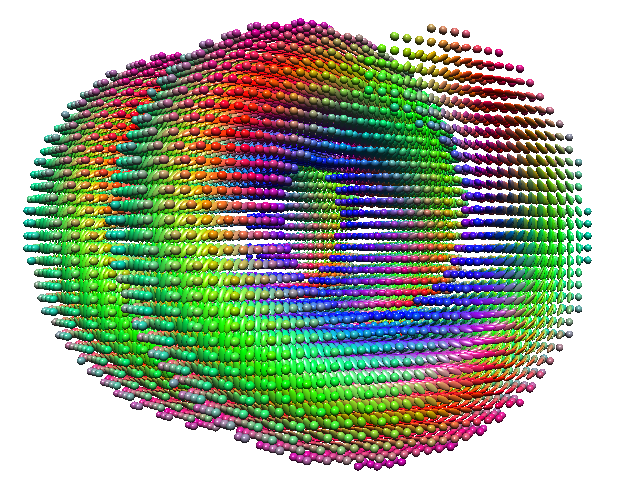
\includegraphics[width=0.25\linewidth]{./figures/library/helixAngled1.png}
    }
    \subfloat[][Top View]{
	\label{fig:helix_top}
	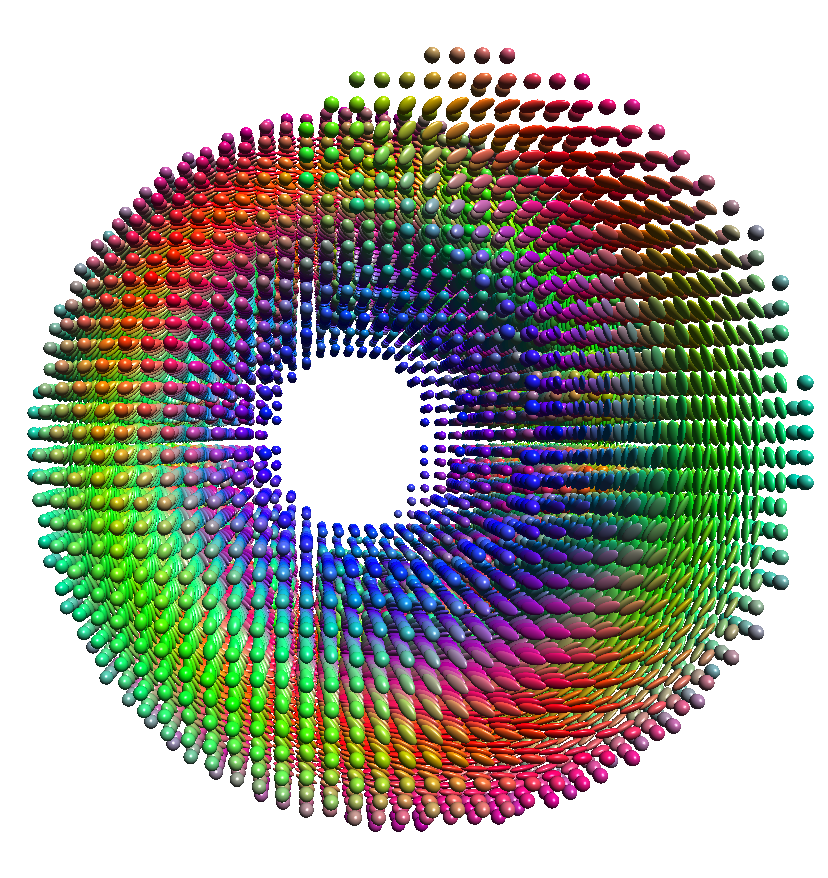
\includegraphics[width=0.25\linewidth]{./figures/library/helixTop1.png}
    }
    \subfloat[][Closeup]{
	\label{fig:helix_close}
	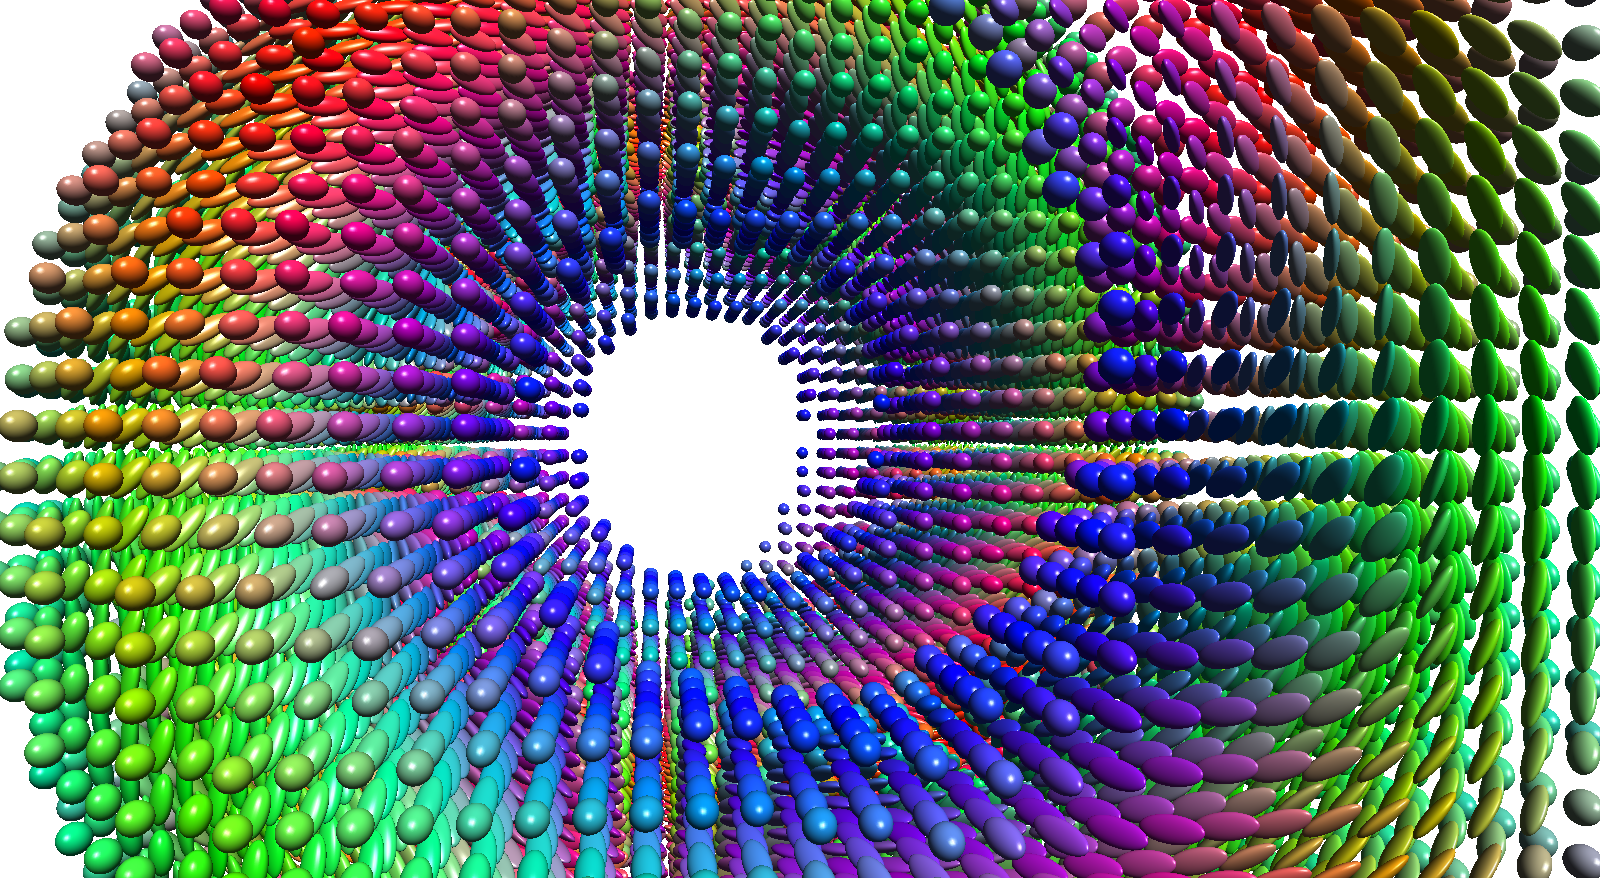
\includegraphics[width=0.25\linewidth]{./figures/library/helixTop2.png}
    }
    \subfloat[][Inside]{
	\label{fig:helix_inside}
	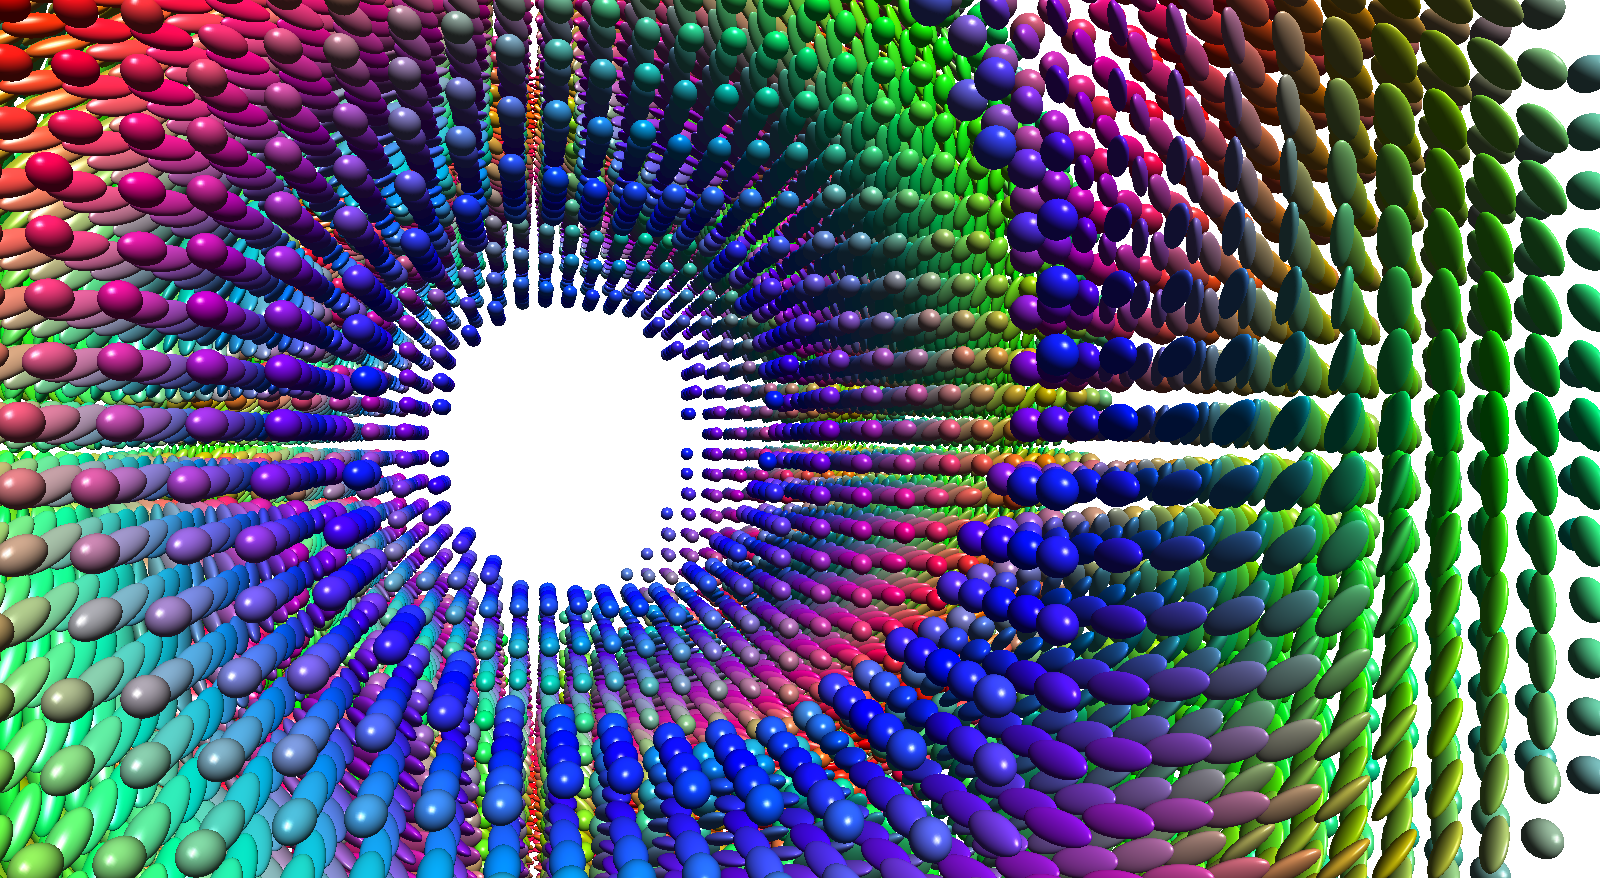
\includegraphics[width=0.25\linewidth]{./figures/library/helixTop3.png}
    }\\
    \caption[3D SPD(3) Volume Visualization of a helix]{Example of the 3D data Visualization of SPD(3) images from different viewpoints.
	\label{fig:helix}
    }
\end{figure}

% subsubsection SPD(3) Visualization (end)
\FloatBarrier
\subsubsection{3D Volume image rendering} % (fold)
\label{ssub:3D Volume image rendering}
The volume image renderer just transforms the data to a 3D texture which is then mapped onto cube rotating about the z-axis.
Plasticity is created by setting the alpha channel of each displayed voxel to the intensity value of the corresponding data voxel, such that dark areas are more transparent.
The following \ref{fig:volume_visualization} shows the rendered volume from different angles.
\begin{figure}[h!]
        \centering
	    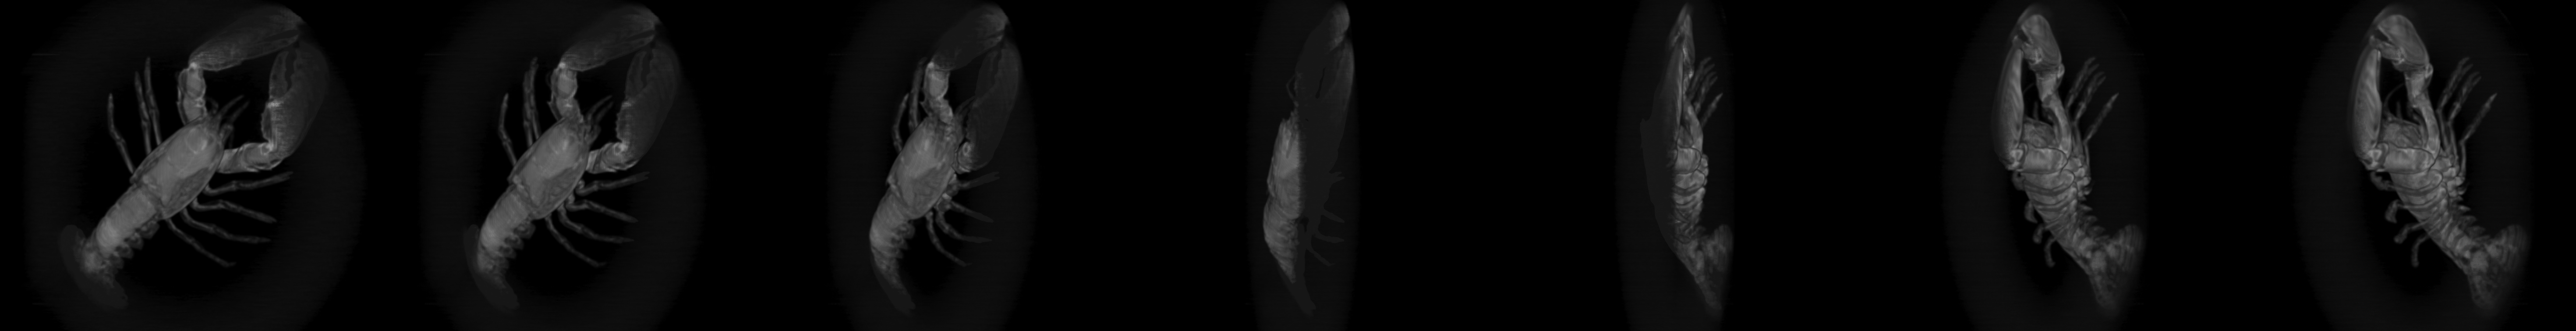
\includegraphics[width=1.0\linewidth]{./figures/library/3dvol_seq.png}
	    \caption[3D Volume image renderer]{3D Volume image using texture based rendering }
	\label{fig:volume_visualization}
\end{figure}
% subsubsection 3D Volume image rendering (end)

% subsection Visualization class (end)

\subsection{Utility functions} % (fold)
\label{sub:Utility function}

\subsubsection{Matrix functions} % (fold)
\label{ssub:Matrix functions}
In the file \texttt{matrix\_utils.hpp} additional matrix functions not included in the Eigen library are implemented.
So far, these are only the methods for the computation of the Fr\'{e}chet derivatives of matrix square root and logarithm, as well as their
Kronecker representations.

% subsubsection Matrix functions (end)

\subsubsection{Function pointers utilities} % (fold)
\label{ssub:Function pointers}
Located in the file \texttt{func\_ptr\_utils.hpp} are some auxiliary functions needed to transform pointers to class member functions
to plain C function pointers requiered by the OpenGL and GLUT library API.
% subsubsection Function pointers (end)

\subsubsection{3D pixel-wise kernels} % (fold)
\label{ssub:3D pixel-wise kernels}
The 3D version of the pixel-wise kernels along with useful tools based on them, for copying or filling 3D images.
% subsubsection 3D pixel-wise kernels (end)

% subsection Utility function (end)


\subsection{External Components} % (fold)
\label{sub:External Components}
Maybe put somewhere else...
\subsubsection{Linear algebra handler: Eigen} % (fold)
\label{ssub:Eigen}

% subsubsection Eigen (end)

\subsubsection{Data storage and processing: Video++} % (fold)
\label{ssub:Video++}

% subsubsection Video++ (end)

% subsection External Components (end)

% section Components (end)


\section{Using TVTML} % (fold)
\label{sec:Using TVTML}

\subsection{Prerequisites} % (fold)
\label{sub:Prerequisites}
The main dependencies of TVTML are the \textit{Eigen} C++ template library for linear algebra and the \textit{Video++} video and image processing library. 
Those libraries, as well as TVMTL's core functionality are provided as header-only libraries. There are, however, some more recommended static libraries
that are recommended to speed up the computation, enable easy I/O or are needed for visualization of the results.
To administer all these different parts and because the header-only libraries require additional compiler flags for the code optimization, TVMTL also relies
on the \textit{CMake} installation tool for installation and compilation of user code using TVMTL. \\

The following lists shows the needed packages for the usage of TVMTL:
\begin{itemize}
    \item CMake ($\geq 2.8.0$)
    \item g++ ($\geq 4.9.1$), any C++14 compatible compiler should also be possible but is untested.
    \item Eigen ($\geq 3.2.5$)
    \item Video++
\end{itemize}

Recommended are also the following packages. They are needed if any of the described extended functionality needs to be used.
\begin{itemize}
    \item OpenCV ($\geq 2.4.9$), for image input and output, edge detection for inpainting
    \item CGAL ($\geq 4.3$), for first guess interpolation during inpainting
    \item OpenGL ($\geq 7.0$), for visualizations of SPD, SO and any 3D data
    \item SuiteSparse ($\geq 4.2.1$), faster parallel sparse solver for the linear system in the IRLS algorithm
\end{itemize}
% subsection Prerequisites (end)

\subsection{Installation} % (fold)
\label{sub:Installation}

% subsection Installation (end)

\subsection{Compilation of own projects using CMake} % (fold)
\label{sub:CMakeCompilation}

% subsection Compilation of own projects using CMake (end)

\subsection{Tutorial and typical use cases} % (fold)
\label{sub:Tutorial and typical use cases}
The basic process of using the library is to explicitly specify the necessary template parameters for all needed components. 
For the sake of compactness and readability this should be done using \texttt{typedef}s. In the next step one can then
instantiate the classes and start implementing.\\

\subsubsection{Image denoising, vectorial color model} % (fold)
\label{ssub:Image denoising, vectorial color model}
As a first example we show the denoising of a simple color picture using the IRLS minimizer. In a first step the necessary classes need to be included. For the sake of shortening the 
code we also switch to the \texttt{tvmtl} namespace of the library. \\
\cppinline
\begin{lstlisting}[label=code:tut_include,caption={Inclusion of library headers}]
#include "../core/algo_traits.hpp"
#include "../core/tvmin.hpp"

using namespace tvmtl;
\end{lstlisting}

Next, we specify the manifold type and data type we want to use, in this case Euclidian $\mathbb{R}^3$ and a corresponding 2D image container\\

\cppinline
\begin{lstlisting}[label=code:tut_typedef,caption={Specification of manifold and data type}]
typedef Manifold< EUCLIDIAN, 3 > mf_t;
typedef Data< mf_t, 2> data_t;
\end{lstlisting}

Note that the data type must be specified using the \textit{fully} specialized manifold class type we defined in the line before.\\
Our data type is now ready for work such that we can read the input data in the next few lines.\\

\cppinline
\begin{lstlisting}[label=code:tut_data,caption={Initialization and input of image data}]
data_t myData=data_t();		// Creating the data object
myData.rgb_imread(filename);	// Reading an image file, filename is a const char*
\end{lstlisting}

After the data object is ready we must specify the functional we want to use, which we choose to be first order TV, isotropic and 2D. Again,
also the fully specified manifold and data class types need to be given as template parameter. The last template parameter, the dimension of the data, 
has default value $2$ and can also be omitted in this case.\\

\cppinline
\begin{lstlisting}[label=code:tut_func,caption={Defining the functional and setting parameters}]
typedef Functional<FIRSTORDER, ISO, mf_t, data_t, 2> func_t;

func_t myFunc(lambda, myData);  // Creation of the functional object
myFunc.seteps2(1e-10);		// Specify the epsilon parameter 
\end{lstlisting}

For the instantiation of the functional we need to pass the $\lambda$ for our functional as well as our newly created data object. The \texttt{seteps2} method
sets the value of $\epsilon^2$ for the reweighting computation. In case of the proximal point algorithm it should be set to zero.\\

\cppinline
\begin{lstlisting}[label=code:tut_data,caption={Choosing the minimizer, smoothing and minimization}]
typedef TV_Minimizer< IRLS, func_t, mf_t, data_t, OMP, 2> tvmin_t;

tvmin_t myTVMin(myFunc, myData);// Creation of minimizer object

myTVMin.smoothening(5);		// smoothing to obtain better starting value
myTVMin.minimize();		// Starts the minimization
\end{lstlisting}

Finally we choose the minimizer we want to use, in this case IRLS, and pass functional, manifold and data types as template parameters. The OMP parameter is not fully implemented yet 
and is supposed to provide choice between different parallelization schemes or also completely serial computation. The last parameter again has default value $2$ and describes the 
dimension of the data.\\
The complete listing of this example can be found in \ref{ap:example_listings}.
% subsubsection Image denoising, vectorial color model (end)

\subsubsection{Colorization using color inpainting} % (fold)
\label{ssub:Color inpainting}
In the following we show a more complicated example: Recolorization of an image where most($\approx$99\%) \textit{color} information has been removed. This means that this
problem is defined on the product manifold $S^2\times \mathbb{R}$, optimization however will only take place on $S^2$ while the $\mathbb{R}$ data part is only needed to obtain
edge information. We also three auxiliary functions (\texttt{removeColor}, \texttt{DisplayImage}, \texttt{recombineAndShow}) here that are not shown in the code snippets but
will be included in the full listing in the appendix \ref{ap:example_listing}. This time, we start by also obtaining some of the minimization parameters from the command line:\\

\cppinline
\begin{lstlisting}[label=code:tut2_init,caption={Include library files and read parameters from standard input}]
#include <iostream>
#include <string>
#include <cmath>

#include <opencv2/highgui/highgui.hpp>
#include "../core/algo_traits.hpp"
#include "../core/data.hpp"
#include "../core/functional.hpp"
#include "../core/tvmin.hpp"

#include <vpp/vpp.hh>
#include <vpp/utils/opencv_bridge.hh>

using namespace tvmtl;

int main(int argc, const char *argv[])
{
    if (argc < 3){
	std::cerr << "Usage : " << argv[0] << " image [lambda] [threshold]" << std::endl;
	return 1;
    }

    double lam=0.01;
    double threshold=0.01;

    if(argc == 4){
	lam=atof(argv[2]);
	threshold=atof(argv[3]);
    }   

    std::string fname(argv[1]);

    //...

}
\end{lstlisting}
Here \texttt{threshhold} defines the percentage of color information that remains in the picture.\\
In the next step, we again define the necessary type definitions for manifold and data classes and create our data objects.

\cppinline
\begin{lstlisting}[label=code:tut2_mfdata,caption={Manifold and Data class type definitions and instantiation}]
// typdefs
typedef Manifold< SPHERE, 3 > spheremf_t;  // S^2
typedef Manifold< EUCLIDIAN, 1 > eucmf_t;  // R
 
typedef Data< spheremf_t, 2> chroma_t;	// Chromaticity part
typedef Data< eucmf_t, 2> bright_t;	// Brightness part

// Instantiation
chroma_t myChroma=chroma_t();
bright_t myBright=bright_t();
\end{lstlisting}

When the data containers are ready we need to read the input picture, extract color and brightness information and store it in the respective objects.
This problem is basically a color inpainting problem but we do not want the reconstructed color to blur across edges in the picture. This can be solved
by making use of the edge weights array that is stored together with the image. We will detect edged in the brightness part of the picture and and
use those edges in the Chromaticity denoising procedure.\\
Finally, we will remove the color in the following way: Create a random inpainting matrix where the probability a certain pixel is set to false is given
by the \texttt{threshold} variable and then replace every RGB pixel by the mean of its three color components (those pixels are basically gray scale then).\\
The necessary steps are shown in the next listing

\cppinline
\begin{lstlisting}[label=code:tut2_edgeandcolorremoval,caption={Color and brightness input, edge detection and color removal}]
myBright.rgb_readBrightness(argv[1]);	// Extract brightness from filename argv[1]
myBright.findEdgeWeights();		// Detect edges and store in matrix

myChroma.rgb_readChromaticity(argv[1]); // Extract chromaticity from filename argv[1]
myChroma.inpaint_=true;			// Turn inpainting on
myChroma.setEdgeWeights(myBright.edge_weights_); // Initiliaze chromaticity part edges with brightness part edges
myChroma.createRandInpWeights(threshold);   // Create random inpainting matrix
removeColor(myChroma, myBright);	    // Remove color

// Recombine chromaticity and brightness and show the colorless image
recombineAndShow(myChroma, myBright, "colorless_"+fname, "Colors removed Picture");
\end{lstlisting}

The next part works almost exactly as in the last example. We define functional, set its parameters, then define the minimizer. The only difference is that
we have to run \texttt{first\_guess} before the minimization.\\

\cppinline
\begin{lstlisting}[label=code:tut2_functionalmin,caption={Functional and minimizer definition, first guess and minimization}]
typedef Functional<FIRSTORDER, ISO, spheremf_t, chroma_t> cfunc_t;
typedef TV_Minimizer< IRLS, cfunc_t, spheremf_t, chroma_t, OMP > ctvmin_t;

cfunc_t cFunc(lam, myChroma);	    // create functional object
cFunc.seteps2(1e-10);		    // set eps^2 parameter

ctvmin_t cTVMin(cFunc, myChroma);   // create minimizer object
cTVMin.first_guess();		    // first guess

std::cout << "Start TV minimization..." << std::endl;
cTVMin.minimize();		    

// Recombine Brightness and Chromaticity parts of recolored Picture
recombineAndShow(myChroma, myBright, "recolored_"+fname, "Recolored Picture");
\end{lstlisting}

Some visual results of the above code are also shown in section \ref{sub:colorinpainting}.



% subsubsection Color inpainting (end)

\subsubsection{3D DT-MRI data denoising and visualization} % (fold)
\label{ssub:dti_tut}
As a final example we choose a more complicated manifold, SPD(3) in this case, as well as 3D data to also demonstrate the use of the visualization classes. Moreover, we use
the proximal point algorithm in this example. The CSV reader just reads a list of pixels where the numerical values comprising the pixel are stored comma-separated one pixel
per line. The CSV files has no header such that we provide the dimensions as command line parameters.

\cppinline
\begin{lstlisting}[label=code:tut3_init,caption={Initialization}]
#include <iostream>
#include <cstdlib>
#include <string>
#include <sstream>

#include "../core/algo_traits.hpp"
#include "../core/data.hpp"
#include "../core/functional.hpp"
#include "../core/tvmin.hpp"
#include "../core/visualization.hpp"

int main(int argc, const char *argv[])
{       
    int nz, ny, nx;
    nz = std::atoi(argv[2]);
    ny = std::atoi(argv[3]);
    nx = std::atoi(argv[4]);

    std::stringstream fname;
    std::string nfname;
    fname << "dti3d" << nz << "x" << ny << "x" << ny << ".png";
    nfname = "noisy_" + fname.str();
    
    // ...

    return 0;    
}
\end{lstlisting}
	
Since the meaning of the individual components should be clear by now by do all the necessary type definitions at once in the next listing\\
\cppinline
\begin{lstlisting}[label=code:tut3_typdefinitions,caption={Type definitions, Visualization type}]
using namespace tvmtl;

typedef Manifold< SPD, 3 > mf_t;
typedef Data< mf_t, 3> data_t;
typedef Functional<FIRSTORDER, ANISO, mf_t, data_t, 3> func_t;
typedef TV_Minimizer< PRPT, func_t, mf_t, data_t, OMP, 3 > tvmin_t;
typedef Visualization<SPD, 3, data_t, 3> visual_t;
\end{lstlisting}

The only innovation is the aforementioned Visualization class. The first $3$ in its template parameter list is the embedding dimension of the manifold 
and the last $3$ denotes the dimension of the data. Note that we needed to specify it for the functional and minimizer classes as well because the default value is $2$. 
The remaining parameters specify the manifold type via an enumeration constant (in the same way one specifies it for the Manifold class) and the data type via a fully
specialized data class type.\\
Before we start the minimization we want to display the original noisy data and eventually save it to a file once we have found a nice viewing angle in the rendering window.
The necessary steps are as follows:\\

\cppinline
\begin{lstlisting}[label=code:tut3_rendernoisyimg,caption={Data input and displaying the noisy data}]
data_t myData = data_t();   // Create data object
myData.readMatrixDataFromCSV(argv[1], nz, ny, nx); // Read from CSV file

visual_t myVisual(myData);  // Create visualization object
myVisual.saveImage(nfname); // Specify file name to save a screenshot

std::cout << "Starting OpenGL-Renderer..." << std::endl;
myVisual.GLInit("SPD(3) Ellipsoid Visualization"); // Start the Rendering
\end{lstlisting}

In the last step we create functional and minimizer class, perform the minimization and display the denoised data again.

\cppinline
\begin{lstlisting}[label=code:tut3_rendernoisyimg,caption={Minimization and final rendering}]
double lam=0.7;
func_t myFunc(lam, myData); // Functional object
myFunc.seteps2(0);  // eps^2 should be 0 for PRPT

tvmin_t myTVMin(myFunc, myData); // Minimizer object

std::cout << "Start TV minimization.." << std::endl;
myTVMin.minimize();

std::string dfname = "denoised(prpt)_" + fname.str();
myVisual.saveImage(dfname); // Specify name for denoised image

std::cout << "Starting OpenGL-Renderer..." << std::endl;
myVisual.GLInit("SPD(3) Ellipsoid Visualization"); // Render
\end{lstlisting}

The resulting picture for this example are also shown in \ref{sub:3DDTMRIdata}.


% subsubsection DT-MRI data denoising and visualization (end)

% subsection Tutorial and typical use cases (end)


% section Using TVTML (end)


\end{chapter}
